\section{Experiments}
\begin{figure*}[htbp]
	\centering
	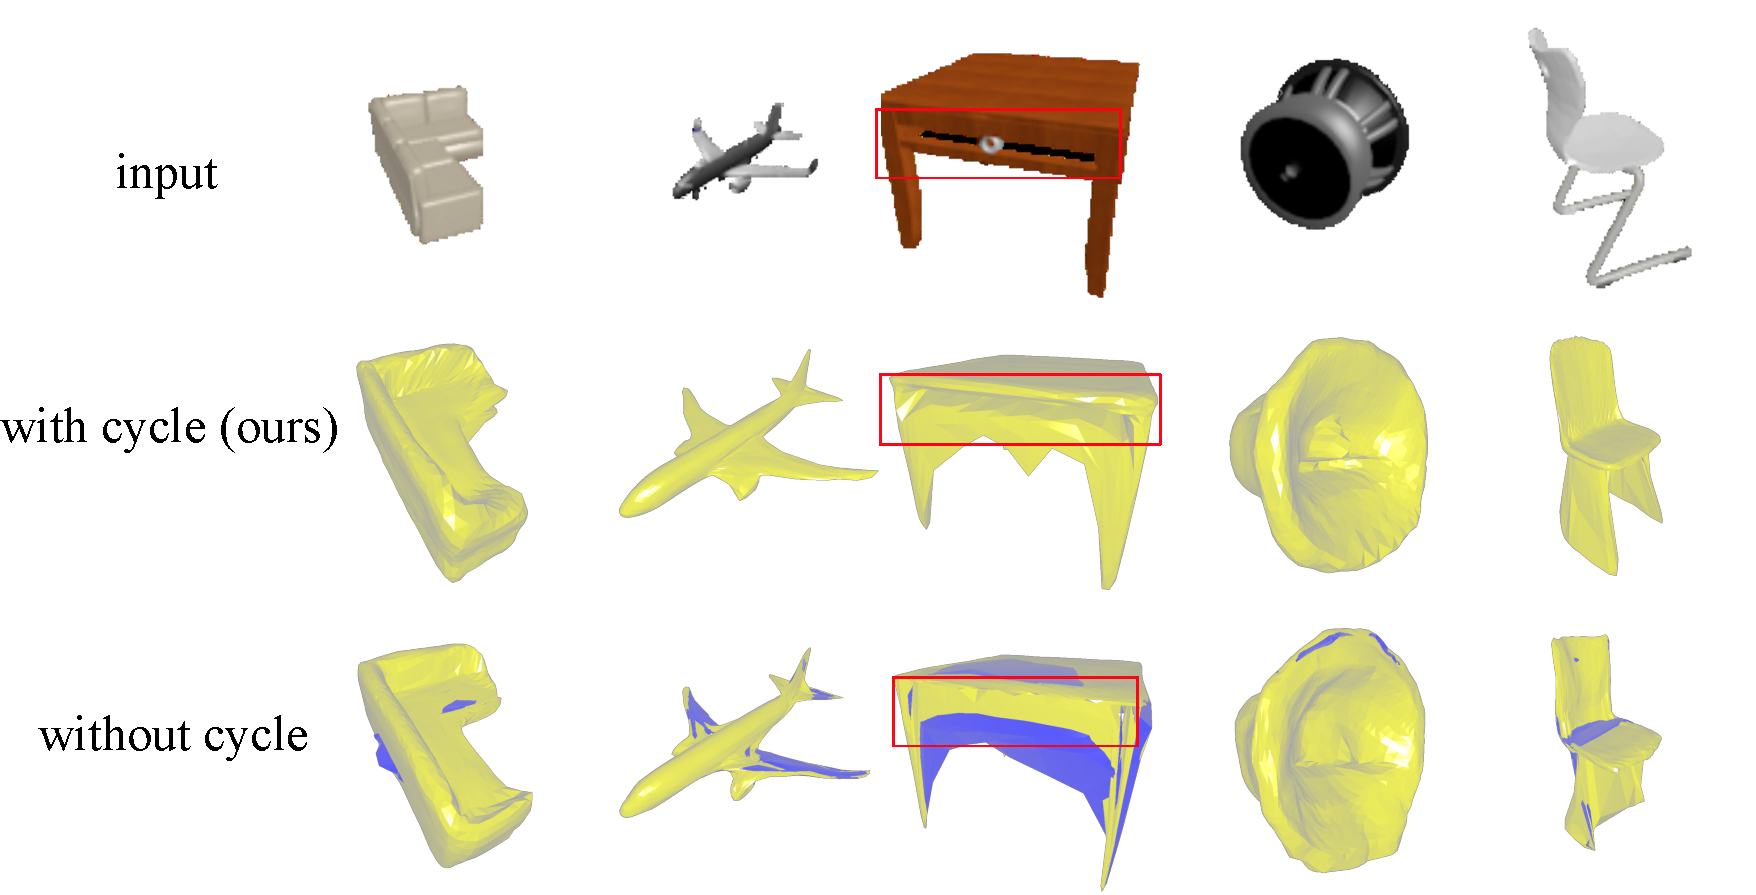
\includegraphics[width=\linewidth]{img/atlas/svr}
	\caption{Cycle regularization on AtlasNet: All the visualized cases here are selected from the test set of AtlasNet. Some meshes' view direction are manually adjusted to better expose the differences. The red rectangles are highlighting a case (the table) in which more details are preserved than the original network because we are enforcing the surface to be free of self-intersection with our cycle regularization term}
	\label{fig:svr}
\end{figure*}

\noindent{\textbf{Data}} To fairly evaluate the effect of cycle regularization, we use the datasets released by AtlasNet and Pixel2Mesh respectively. Their model sets are both subsets of ShapeNet\cite{shapenetdata} and they both used the rendered image from \cite{3DR2N2}. The absolute size and position of the models and the sampled points as ground truth are not processed in the same way in these two datasets, which makes it unreasonable to compare them all together. However, this doesn't prevent us to show the effect of our regularization technique separately.

\noindent{\textbf{Mesh generation and visualization}} Since we are addressing a issue regarding the quality of generated mesh, any post-processing used in AtlasNet\cite{atlasnet} are not used in our experiment. All the triangulations are directly transfered from the predefined surface. We do not divide the triangles to get denser vertex either. The meshes from AtlasNet all have 2500 vertices and about 4k faces. The meshes from Pixel2Mesh all have 2466 vertices and 4928 faces.

To better expose the issue we are addressing in this paper, we render the generated mesh in the software MeshLab and use the ``gooch.gdp" in the software as our shader. In such mode the triangles are rendered golden at front and bluish at back. The golden region and bluish region interlacing at surface evidently indicates the self-intersected triangles.

\noindent{\textbf{Evaluation criteria}}
In order to quantitatively evaluate the issue of self-intersection and self-overlap, we count the percentage of self-intersected triangles (``SI") over the total number of triangles. For this evaluation, we provide our code in the supplemental material which can calculate the ``SI" for a input mesh.  
We also use the value of Chamfer distance (``CD") as the original AtlasNet and Pixel2Mesh to evaluate how well the generated mesh approximate the target shape. For the evaluation of Chamfer distance we used the codes that are already implemented by AtlasNet\cite{atlasnet} and Pixel2Mesh\cite{pixel2mesh}.

\begin{table*}
	\caption{Validation error on AtlasNet trained with(\textbf{ours}) and without cycle regularization. Chamfer distance(CD) and percentage of self-intersected(SI) faces are reported}
	\label{tab:seg}
	\centering
	\begin{tabular}{c|rc|rc|rc|rc|}
		\multirow{2}{*}{CD,SI} &\multicolumn{4}{c|}{AE-sphere}&\multicolumn{4}{c|}{SVR-sphere}\\
		\cline{2-9}
		~& \multicolumn{2}{c|}{without-cycle} & \multicolumn{2}{c|}{ours} & \multicolumn{2}{c|}{without-cycle} & \multicolumn{2}{c|}{ours} \\
		\hline
		cellphone&1.3,&0.53\%&1.4,&3.4e-3\%&3.8,&1.4\%&3.7,&2.7e-4\%\\
		watercraft&1.5,&2.3\%&1.8,&6.8e-4\%&4.3,&7.4\%&4.3,&2.6e-4\%\\
		monitor&1.8,&1.8\%&2.0,&9.8e-4\%&6.9,&3.4\%&6.5,&9.8e-4\%\\
		car&1.8,&0.52\%&1.8,&8.0e-4\%&3.9,&0.47\%&3.8,&1.8e-3\%\\
		couch&1.9,&2.5\%&1.9,&8.8e-4\%&5.1,&2.0\%&4.9,&1.7e-3\%\\
		cabinet&2.0&2.3\%&2.2,&1.2e-2\%&5.3,&3.6\%&5.2,&4.3e-3\%\\
		lamp&2.7,&14\%&3.4,&5.5e-2\%&13.2,&19\%&13.1,&2.0e-2\%\\
		plane&1.0,&18\%&1.2,&1.9e-3\%&2.6,&18\%&2.6,&2.9e-3\%\\
		speaker&2.9,&0.77\%&2.9,&1.1e-3\%&10.2,&1.7\%&9.6,&3.1e-4\%\\
		bench&1.3,&11\%&1.6,&7.4e-3\%&4.0,&12.3\%&3.9,&1.6e-2\%\\
		table&1.7,&12\%&2.0,&2.1e-2\%&4.9,&10.7\%&4.8,&1.79e-5\%\\
		chair&1.9,&12\%&2.1,&2.7e-2\%&5.3,&10.9\%&5.3,&2.3e-2\%\\
		firearm&0.7,&4.9\%&0.9,&2.1e-3\%&2.2,&18.2\%&2.2,&1.2e-3\%\\
		\hline
		mean &1.7,&8.5\%&1.9,& 1.3e-2\% &5.2,&9.6\%&5.0,&1.2e-2\%\\
		
	\end{tabular}
\end{table*}

\subsection{Visualize deformation process}
\label{subsec:deform}
In this subsection, we visualize the deformation process, providing a more intuitive view into the effect of our cycle regularization term. Being free of self-intersection is a rather geometric prior for surface mesh than a semantic one, therefore for the visualization in this section we do not involve any semantic networks and show the effect of our proposed technique in a pure shape deforming manner. In other words, we optimize the same loss function as in Equ.~(\ref{equ:atlascycle}), but do not use semantic networks (neither ResNet-18\cite{resnet} nor PointNet\cite{pointnet}) to generate the latent shape representation $\mathbf{s}$. We treat $\mathbf{s}$ as 1024 free variables. We initialize the parameters $\theta_f,\theta_g,\mathbf{s}$ randomly and use gradient descent method as optimizer. Under such setting, we are deforming a randmly initialized shape (probably start with self-intersection) to a target shape. As in Figure~\ref{fig:opt}, the case of two target shapes (downloaded from the Internet) are shown. In these two cases, after few iterations our cycle regularization term take effect. It not only keep the mapping injective in optimization but also correct the self-intersection from the initialization.

\begin{figure}[htbp]
	\centering
	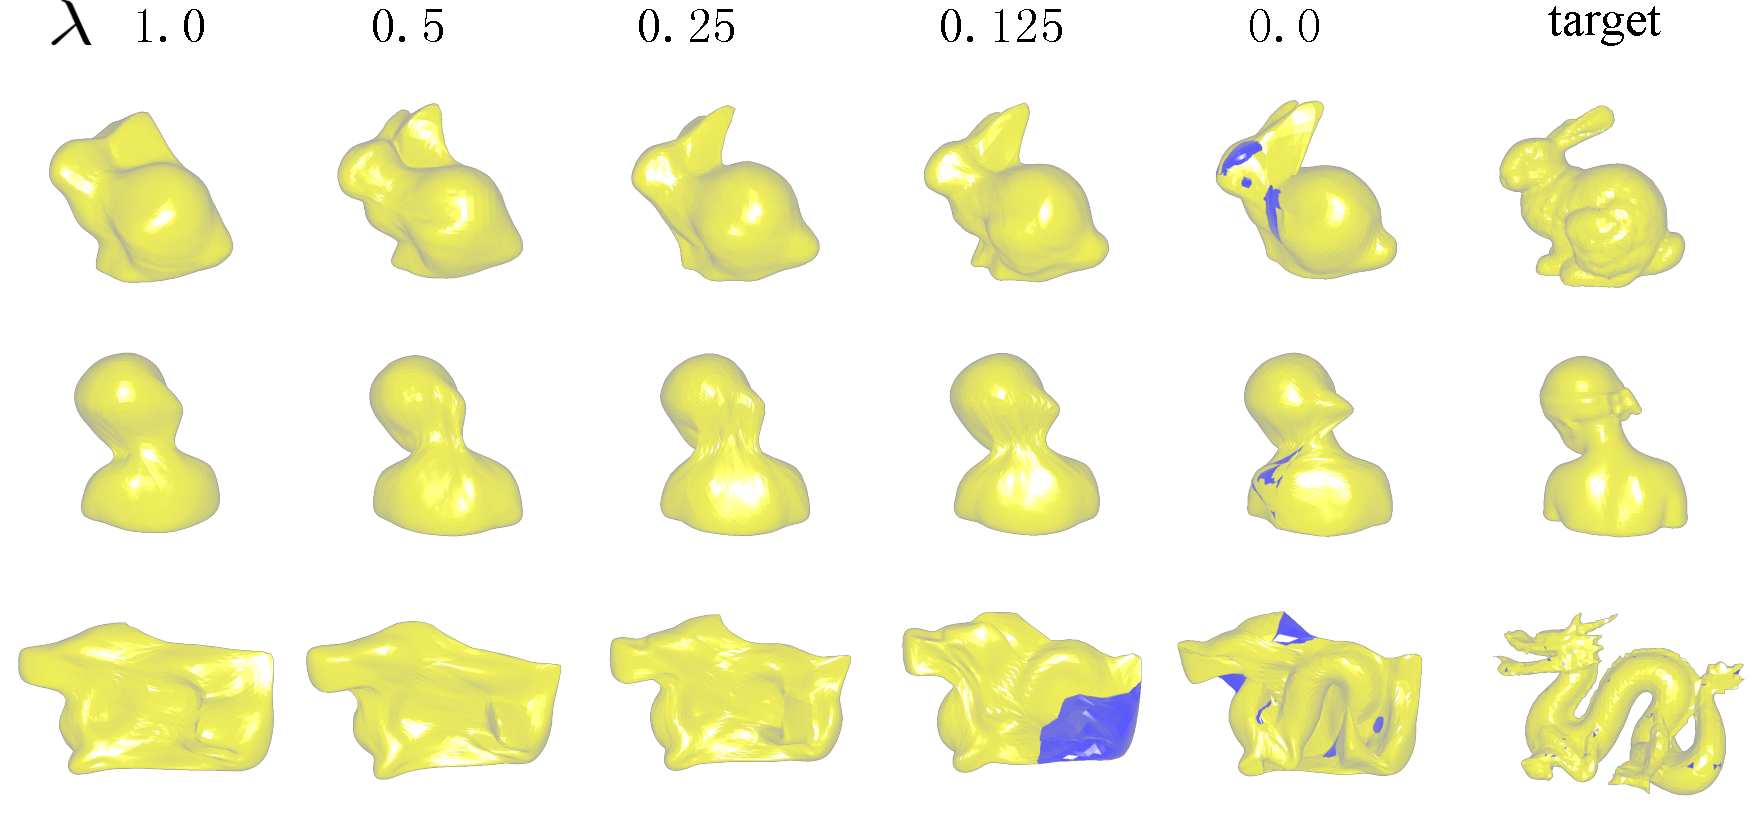
\includegraphics[width=\linewidth]{img/opt/lambda}
	\caption{The choice of $\lambda$: Under the setting in Sec~\ref{subsec:deform}}, we show some results with different choice of $\lambda$}
	\label{fig:lambda}
\end{figure}

As we show in Figure~\ref{fig:lambda}, therefore we use $\lambda=0.25$ as an emperical choice 
\subsection{Cycle regularization with AtlasNet}


		
\todo{train and test atlasnet with and without cycle regularization}

\subsection{Cycle regularization with Pixel2Mesh}

\todo{train and test Pixel2Mesh with and without cycle regularization}

\subsection{Limitations and future work}
